\section{Visualization Layer}\label{sec:ImplementationViz}
\subsection{Multithreading}
The worker thread is implemented with a \code{SystemWorker} class combined with a generic threading system.
% While only one worker thread is ever used in the final program, earlier versions planned to use a few unique workers so a generic system was required.
An \code{IWorkerThread} virtual interface is defined and \code{IWorkerThread_Impl<Worker>} implements this for a specific \code{Worker} class, similar to the Simulation Runners pattern.
% A similar pattern to Simulation Runners is used, where an \code{IWorkerThread} virtual interface is defined and a \code{IWorkerThread\_Impl<Worker>} class implements this for a specific \code{Worker} class.

% The \code{IWorkerThread} class works with a \code{WorkerThreadController} class.
To kick off the worker thread, a \code{WorkerThreadController} writes to a mutex-protected set of input data.
The `work index' of this data is incremented to signal it is new, and a condition variable is signalled to alert the worker thread and begin processing.
Work cannot be enqueued until the thread produces an output, which is sent to the main thread in the same way as before - a mutex is taken to update the output data with the new index, and the condition variable is signalled in case the main thread is waiting for the worker to finish.

\subsection{GPU Work Breakdown}
% \todoref{GPU work breakdown design} showed a coarse breakdown of work between the Viz Compute and Viz Graphics stages, which \cref{fig:VizDataTransform} expands on.
\cref{fig:VizDataTransform} expands on the coarse GPU work breakdown from \cref{sec:Design:Viz:Breakdown}.
Each rectangle represents a piece of memory, and each arrow represents a transformation from input to output via a compute shader, an image layout transfer, or a graphics pipeline.
Most memory is global rather than per-frame, as the system does not run any visualization stages in parallel.
Some per-frame buffers (highlighted in bold) are used to allow race-free accesses at record-time.
These buffers allow user interaction, such as moving the particle emitters and setting the quantity ranges.
% \begin{landscape}
% \thispagestyle{empty}
\pagebreak
\newgeometry{margin=2cm}
\begin{sidewaysfigure}
    \centering
    \makebox[\linewidth][c]{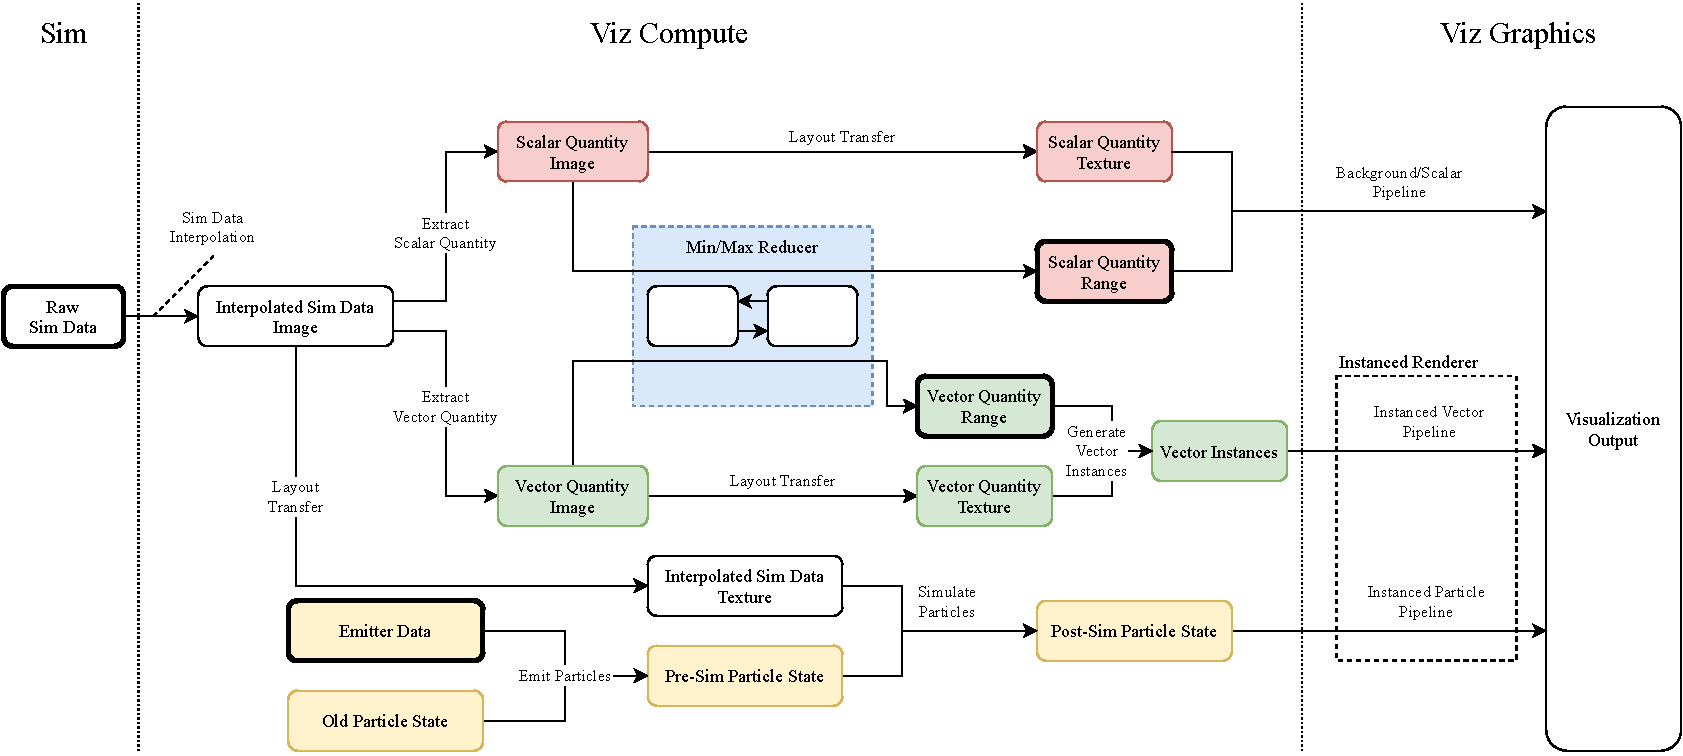
\includegraphics[width=0.9\linewidth]{Ch48Implementation/figures/FinalReport_VizData.pdf}}
    \caption{Data Transformation Diagram showing the data flow for the Visualization}
    \label{fig:VizDataTransform}
\end{sidewaysfigure}
\restoregeometry
\pagebreak
% \end{landscape}

Image layout transfers allow the GPU to optimize access times for an image by changing the format it's stored in.
Images are transferred to the \code{ShaderReadOnlyOptimal} layout (listed as `Texture' rather than `Image' in \cref{fig:VizDataTransform}) for efficient sampling at arbitrary points, and kept in the \code{General} layout when accessed at 2D data arrays (see \cref{fig:VizImageRead} as a comparison).

Memory barriers (not shown in \cref{fig:VizDataTransform}) are inserted between every compute shader to ensure any required data written from a previous shader is visible to the next shader\cite{TheKhronosGroupVulkanSpec}. % Could also be \cite{MaisterVulkanSyncBlog}
% On top of that, each compute shader requires at least one \emph{memory barrier}, to ensure any data written in previous stages is visible to the next stage.
These memory barriers are quite granular, as shown in \cref{fig:VizMemoryBarrier}.

\begin{figure}
    \centering
     \begin{subfigure}[b]{0.49\textwidth}
         \centering
\begin{glslcode}
uniform readonly image2D resultImage;
 // = (u, v, p, isfluid);

// Specify the exact pixel location
ivec2 pxIdx = ivec2(200, 450);
vec4 data = imageLoad(simDataImage, pxIdx);
\end{glslcode}
\caption{Directly}
        %  \label{fig:vizimageLoad}
     \end{subfigure}
     \hfill
     \begin{subfigure}[b]{0.49\textwidth}
         \centering
\begin{glslcode}
uniform sampler2D simDataSampler;
 // = (u, v, p, isfluid);
 
// 50% across, 20% up the image
vec2 sampleAt = (0.5, 0.2);
vec2 velocity = texture(simDataSampler, sampleAt).xy;
\end{glslcode}
\caption{With a Sampler}
        %  \label{fig:vizimagesample}
     \end{subfigure}
  \caption{Reading from an image directly vs. using a sampler.}
    \label{fig:VizImageRead}
\end{figure}
\begin{figure}
    \centering
    \begin{cppcode}
// Make ShaderWrites from the ComputeShader stage available + visible to 
//      IndirectCommandReads in the DrawIndirect stage
fullMemoryBarrier(computeCmdBuffer,
    vk::PipelineStageFlagBits::eComputeShader, vk::PipelineStageFlagBits::eDrawIndirect,
    vk::AccessFlagBits::eShaderWrite, vk::AccessFlagBits::eIndirectCommandRead);
// Make TransferWrites from the Transfer stage available + visible to the
//      ShaderReads in the ComputeShader phase.
fullMemoryBarrier(computeCmdBuffer,
    vk::PipelineStageFlagBits::eTransfer, vk::PipelineStageFlagBits::eComputeShader,
    vk::AccessFlagBits::eTransferWrite, vk::AccessFlagBits::eShaderRead);
    \end{cppcode}
    \caption{Example showing the granularity of Memory Barriers.}
    \label{fig:VizMemoryBarrier}
\end{figure}

\pagebreak
\begin{figure}[t]
    \centering
    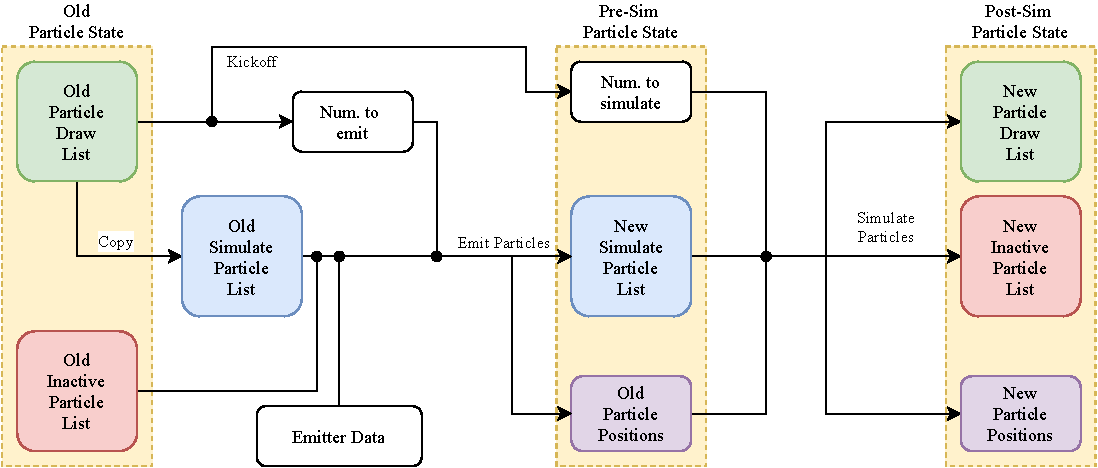
\includegraphics[width=\linewidth]{Ch48Implementation/figures/FinalReport_VizData_Particles.pdf}
    \caption{Breakdown of particle-related GPU work}
    \label{fig:VizDataParticles}
\end{figure}
The particle system implementation in \cref{fig:VizDataTransform} is a simplified view for compactness, \cref{fig:VizDataParticles} shows a full breakdown of this subsystem.
This maintains three growable/shrinkable lists, plus a buffer containing particle positions.
\begin{enumerate}
    \item The Draw list, a list of particle indices to draw on screen
    \item The Inactive list, a list of inactive particle indices
    \item The Simulate list, a list of particle indices which take part in Simulation.
\end{enumerate}
The previous Draw list is the authority on which particles currently exist, and is used for the Kickoff shader to determine how many particles will be emitted/simulated\footnote{This isn't known at record time, because the last frame may still be simulating the particles}.
It is also copied into the Simulate particle list, which is grown by the Emit Particles shader.
The particles are then moved by the Simulate Particles shader as shown in \cref{sec:Research:Viz:Particles}.
These particles are added to the inactive list if out-of-bounds, and the new Draw list otherwise.
% adding particles to the inactive list if they move out of the simulation bounds, and moving all other particles to the new Draw list.

\subsection{Safe CPU/GPU Communication}\label{sec:Impl:Viz:CPUGPUSafety}
Unlike CUDA, the Vulkan API does not provide any means of type-safety when communicating between the CPU and GPU.
If the GPU expects data in a specific structure, it is the CPU's job to create data that fits this structure.
%API user instead of CPU
A naive solution might be to keep a C++ structure definition and a GLSL structure definition, and assume that one matches the other.
This is error-prone as the structures are not automatically kept in sync - if one changes, the other will not, and communication will break down.
This project's approach is to create a GLSL file defining all interoperable structures (\shell{structures.glsl}), and then include it into a C++ header with some extra code to define GLSL types correctly.
Both sides will now use the same structure definitions, which are all defined in exactly one place.
All GLSL code uses the \code{std430} memory layout rules, which closely matches the C++ memory layout, so the structures can be passed directly from the CPU to the GPU safely.

\subsection{Usage in Other Layers}
The \code{VulkanSimApp} class is instantiated by the command-line layer to run the visualization.